\documentclass{article}
\usepackage[a4paper]{geometry}
\usepackage[utf8]{inputenc}

\usepackage{graphicx}
\graphicspath{ {./images_P4/imatges_informe/} }


\title{Informe pràctica 4\\Visió Artificial}
\author{Jordi Olivares Provencio\\Christian José Soler}

\begin{document}

\maketitle

\begin{enumerate}

 \item \textbf{Extracción de descriptores de textura}

 \begin{enumerate}

 \item \textit{Descargar el código para generar un banco de filtros de la Gaussiana (dicho de otra manera: el banco de  filtros de Leung-Malik (LM)) 
 y visualizarlos en una figura. Nota: Fíjate en los comandos imagesc y colorbar. ¿Qué hacen? ¿A qué corresponden los diferentes filtros? ¿Qué valores tienen?}
 
\begin{center}
	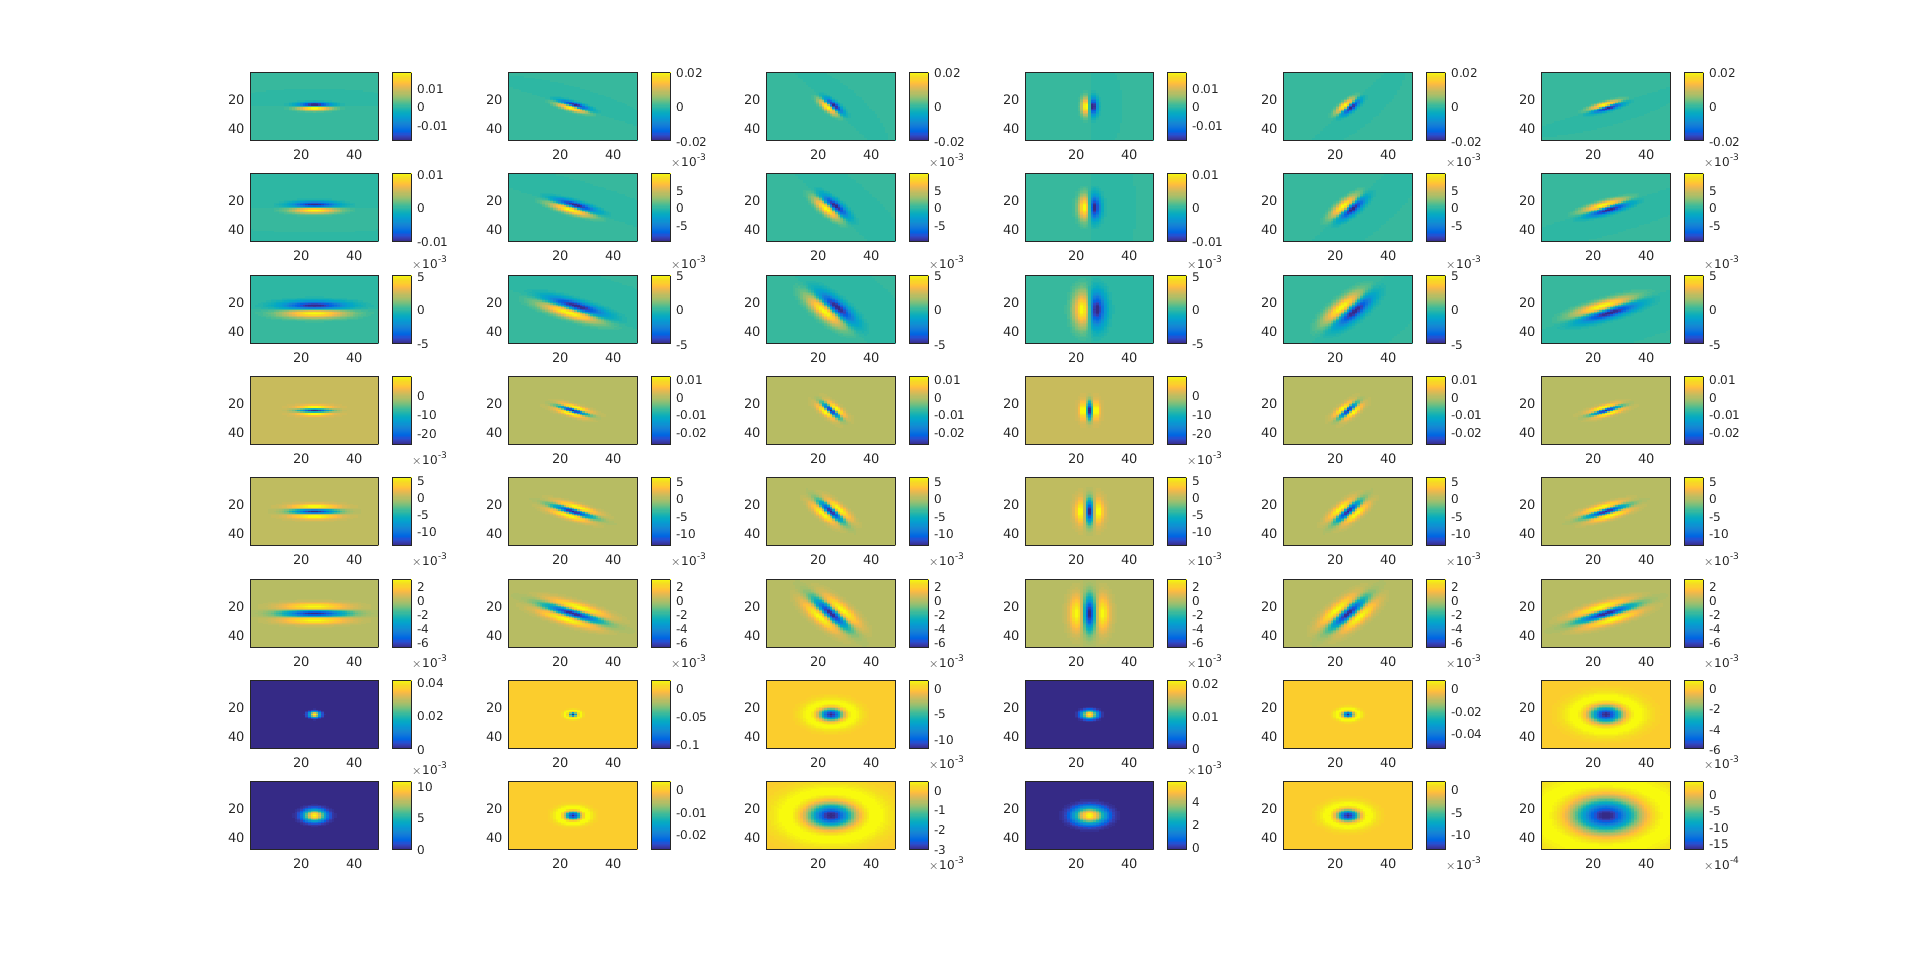
\includegraphics[width=\textwidth]{im411.png}
\end{center}

  Los de arriba son los filtros de la primera derivada de la gaussiana, los del medio la segunda derivada y los de abajo la gaussiana sin derivar. 
  Los valores se muestran en los diagramas, pero básicamente los cambios se notan en el centro del filtro y en la varianza de la distribución usada.
 
 \item \textit{Implementar una  función getFeatures que dada una imagen, construye un descriptor de texturas, donde cada elemento del descriptor es el promedio del 
resultado de la convolución de la imagen con los filtros. ¿Qué dimensión tiene el descriptor? }

 El descriptor tiene dimensión 48.

 \item \textit{Nota: Al buscar la textura de la imagen, no nos importa el color. Por lo tanto, tenéis que convertir la imagen en color a escala de grises. 
 Visualiza el  resultado de la convolución con algunos  filtros. Observa qué  filtros tienen  una  mejor  respuesta  sobre  la  imagen  que  has  escogido  
 y  comenta  el porqué. }

  Escogimos la imagen número forest\_9, es decir, esta:
  
\begin{center}
	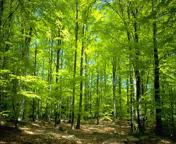
\includegraphics[width=0.3\textwidth]{forest_9.jpg}
\end{center}  

Pasamos los diferentes filtros por la imagen:
 
 \begin{center}
	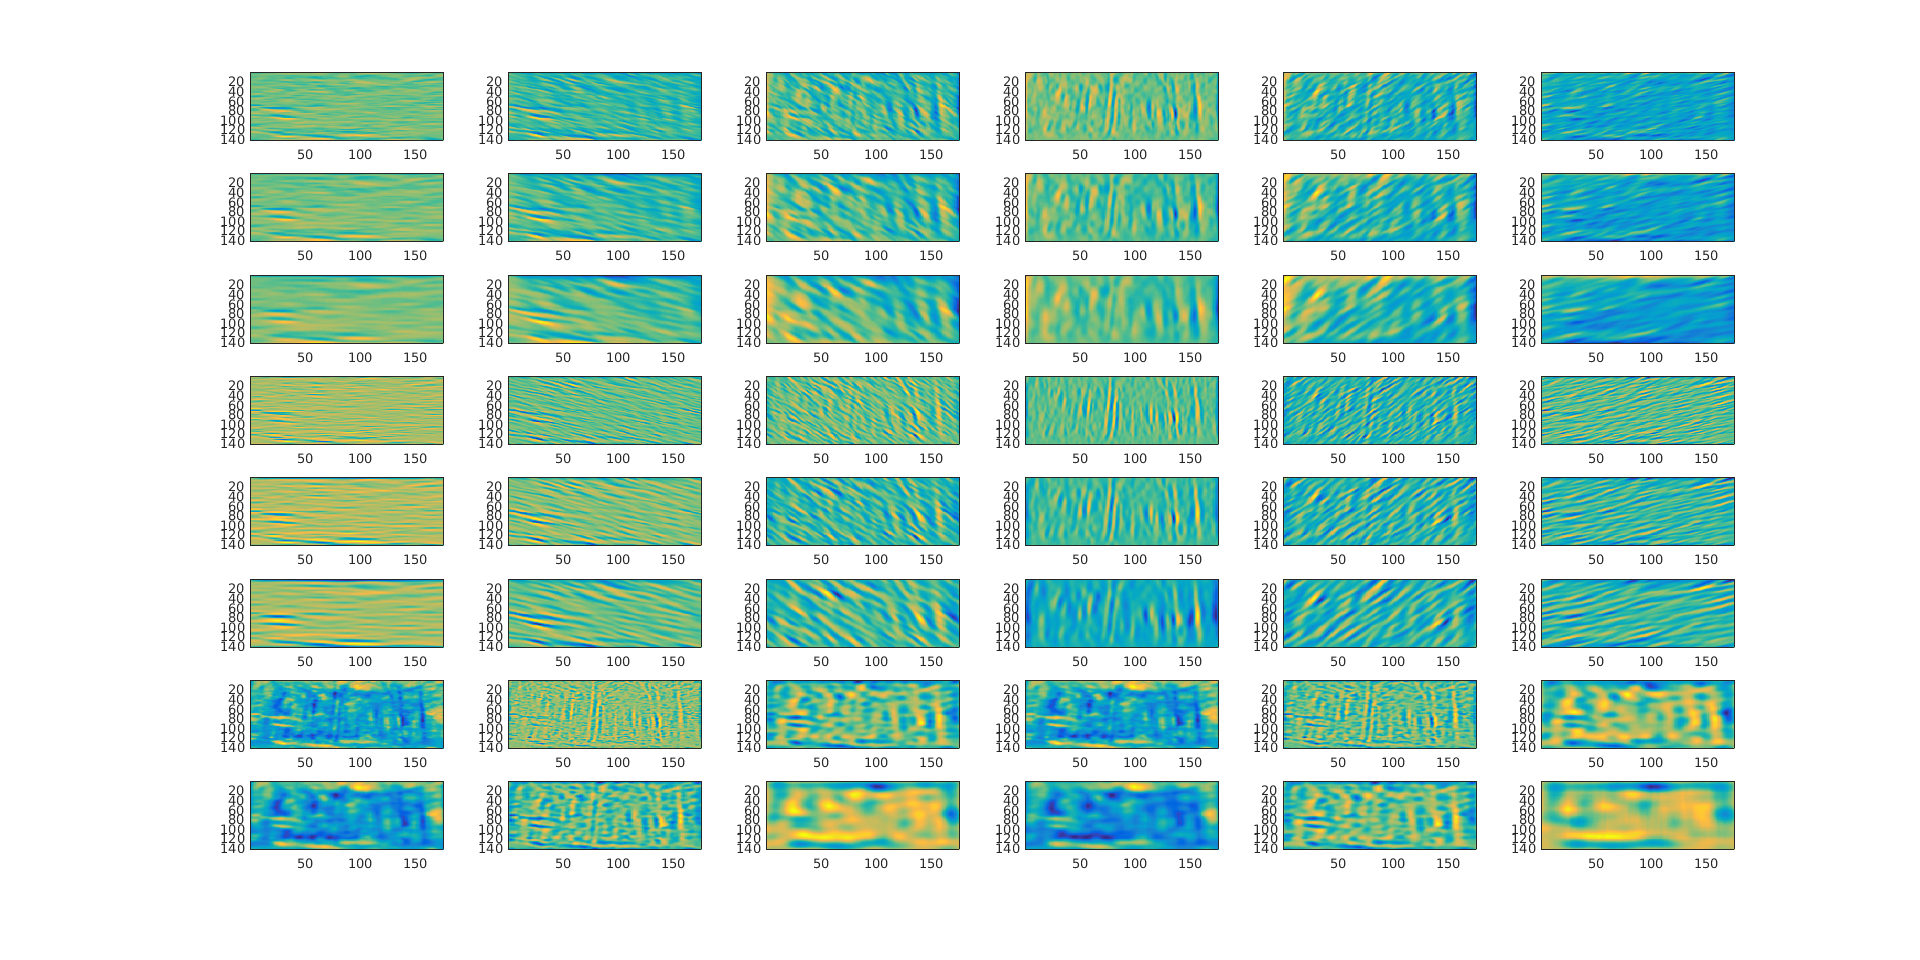
\includegraphics[width=\textwidth]{im412.png}
\end{center}

A primera vista parece que los filtros gaussianos son los más apropiados para detectar los edges. (en concreto los de abajo a la esquina de la izquierda)
  
 \item \textit{Escribir  una  función  getClassFeatures que dado  un  directorio  y  una extensión, lee todas las imágenes del directorio con la extensión dada, 
 calcula sus descriptores de textura (usando getFeatures del 4.1.2) y los guarda en una matriz donde  cada  fila  es  una  imagen  y  cada  columna  una  característica.  Aplicar  esta función para construir tres matrices de descriptores de textura de las 3 clases de imágenes del directorio textureimages facilitado con el enunciado.}

 \item \textit{Escribir una función visualizeFeatures que visualiza en un plot una lista de una o varias características (por ejemplo: [25, 41]) 
 para las imágenes de los tres directorios con un color diferente para cada directorio (help plot).}

\begin{center}
	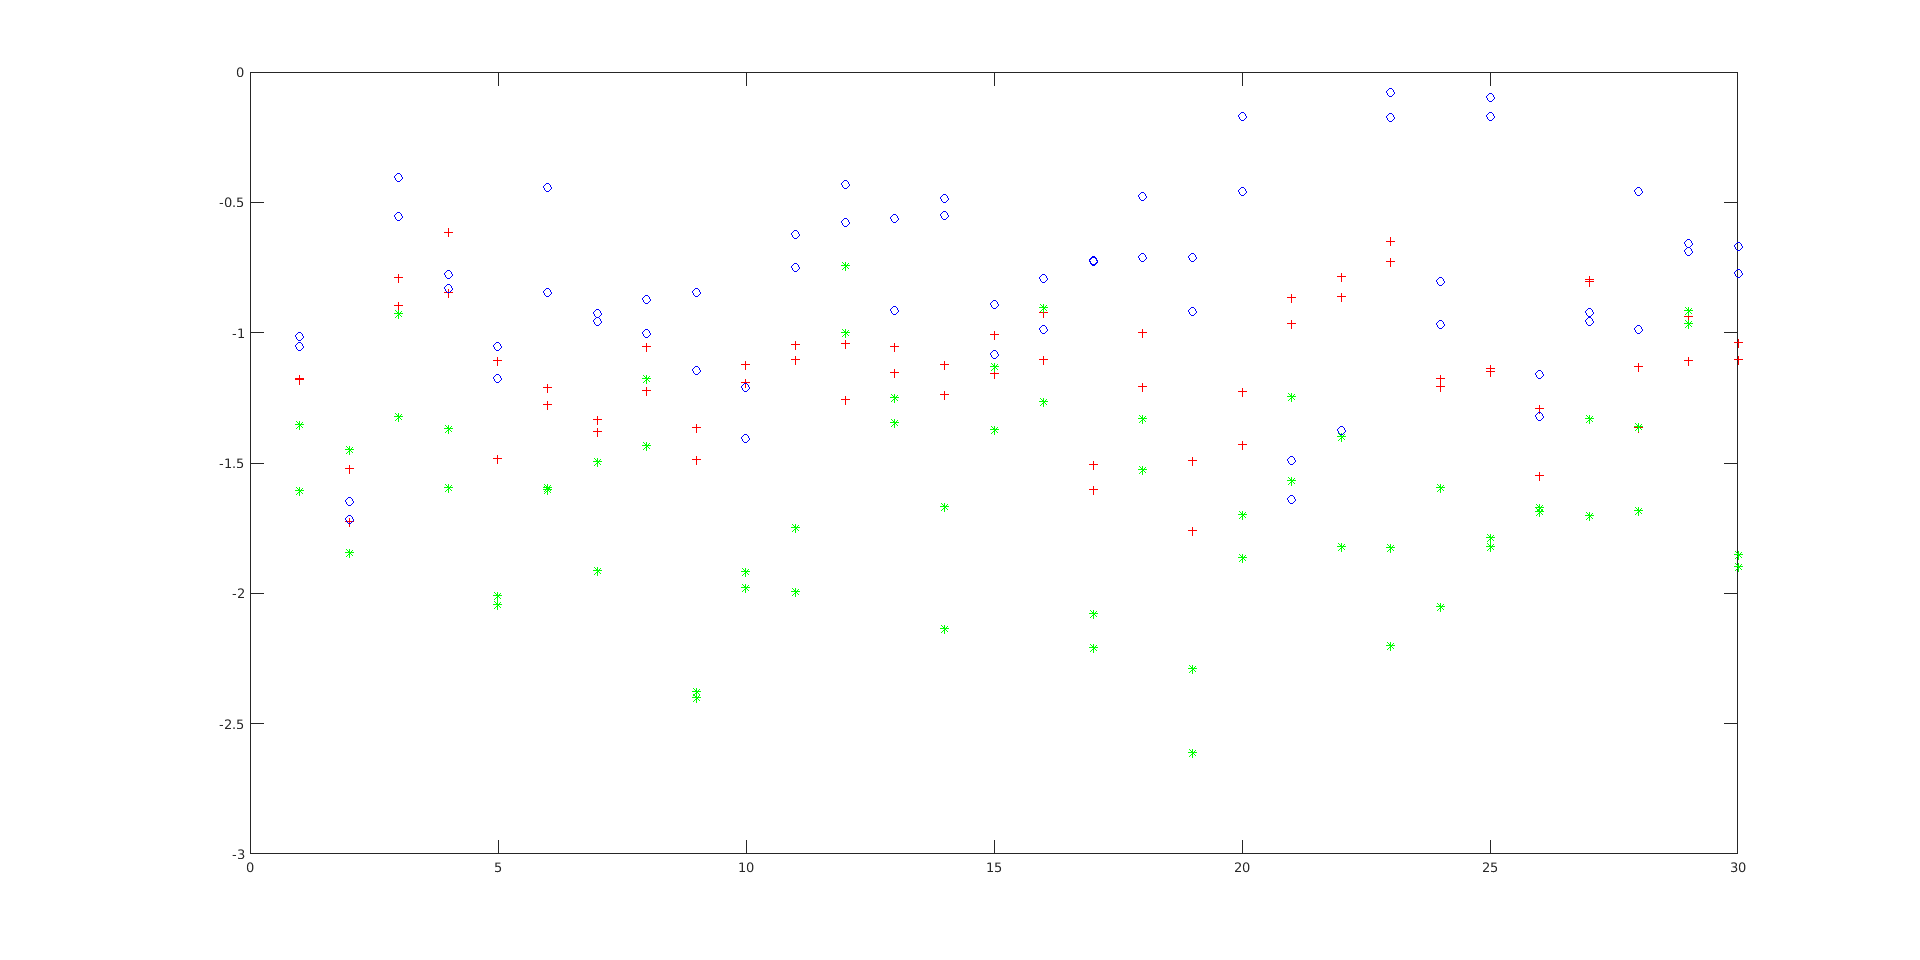
\includegraphics[width=\textwidth]{im414.png}
\end{center}
 
 El rojo son los bosques, verde son edificios y el azul son puestas de sol
 
 \item \textit{Para  cada imagen  de las  tres  clases,  escribir una  función  retrieveKImages que  recupera  y  visualiza  las  k  ($k=9$)  
 imágenes  más parecidas  según  sus descriptores de textura (ver Fig. 4).}
 
 \begin{center}
	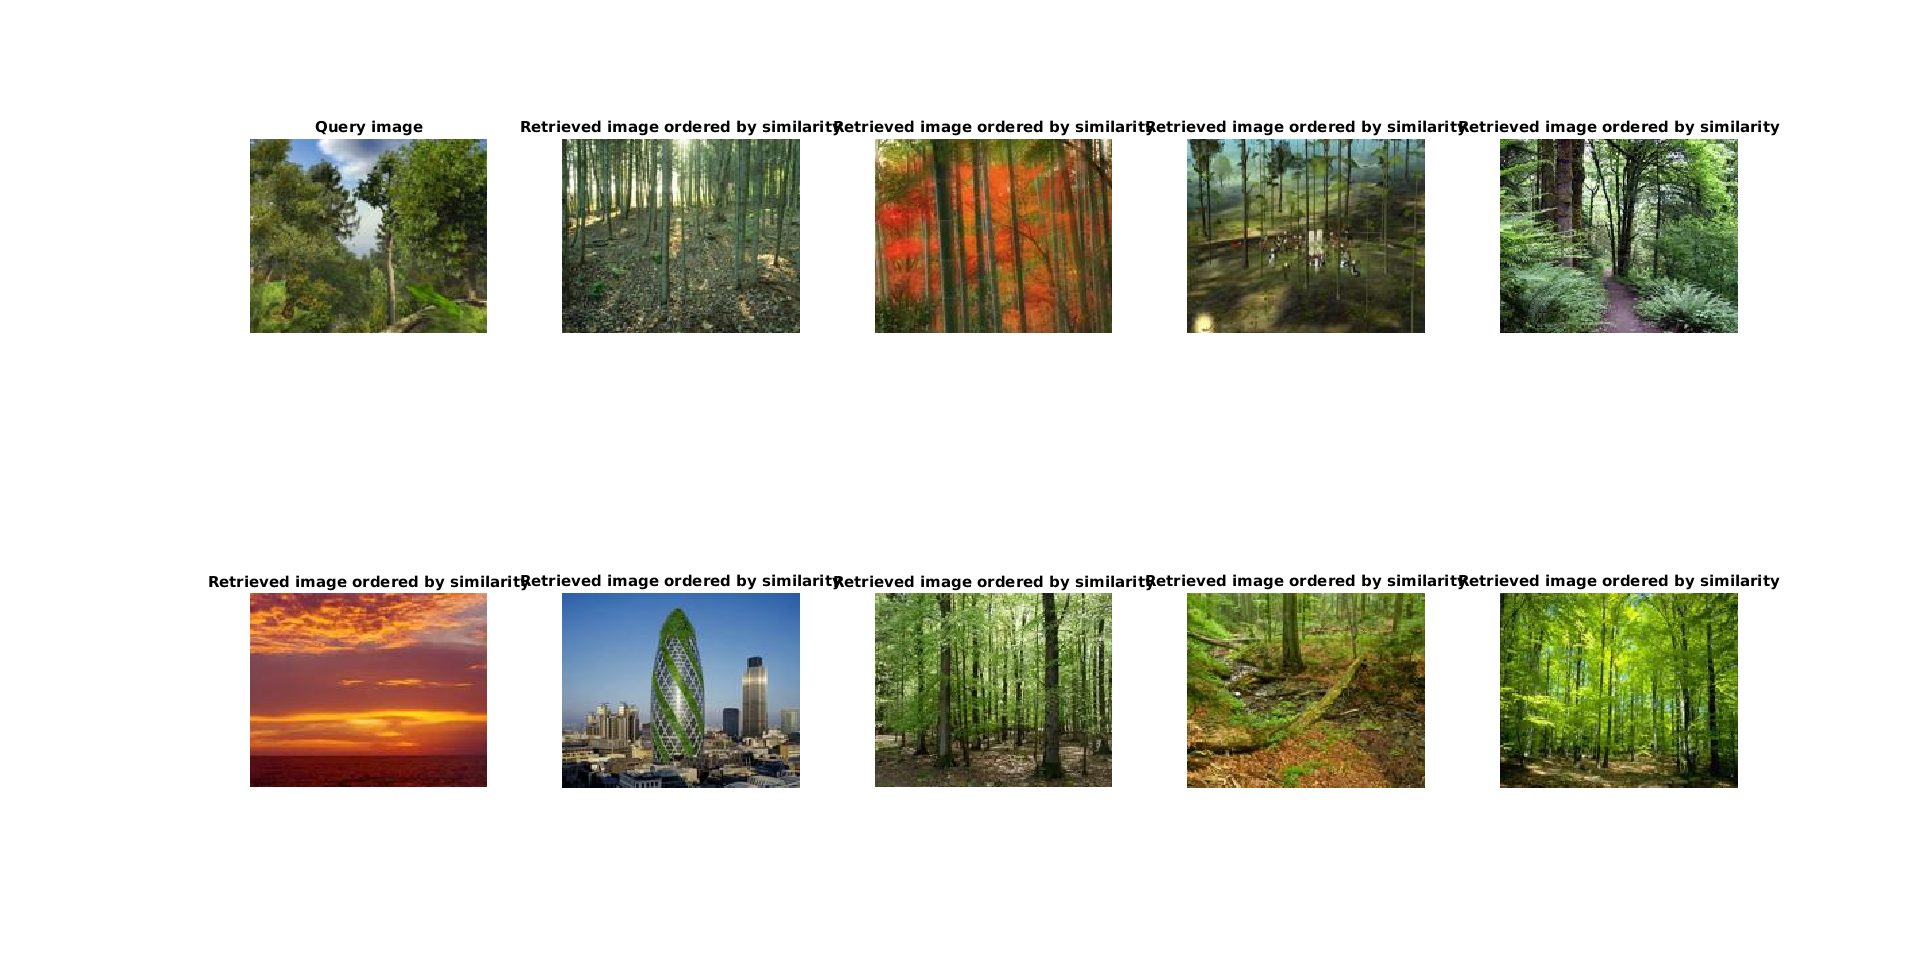
\includegraphics[width=\textwidth]{im415(1)-sinColores.png}
\end{center}

 \begin{center}
	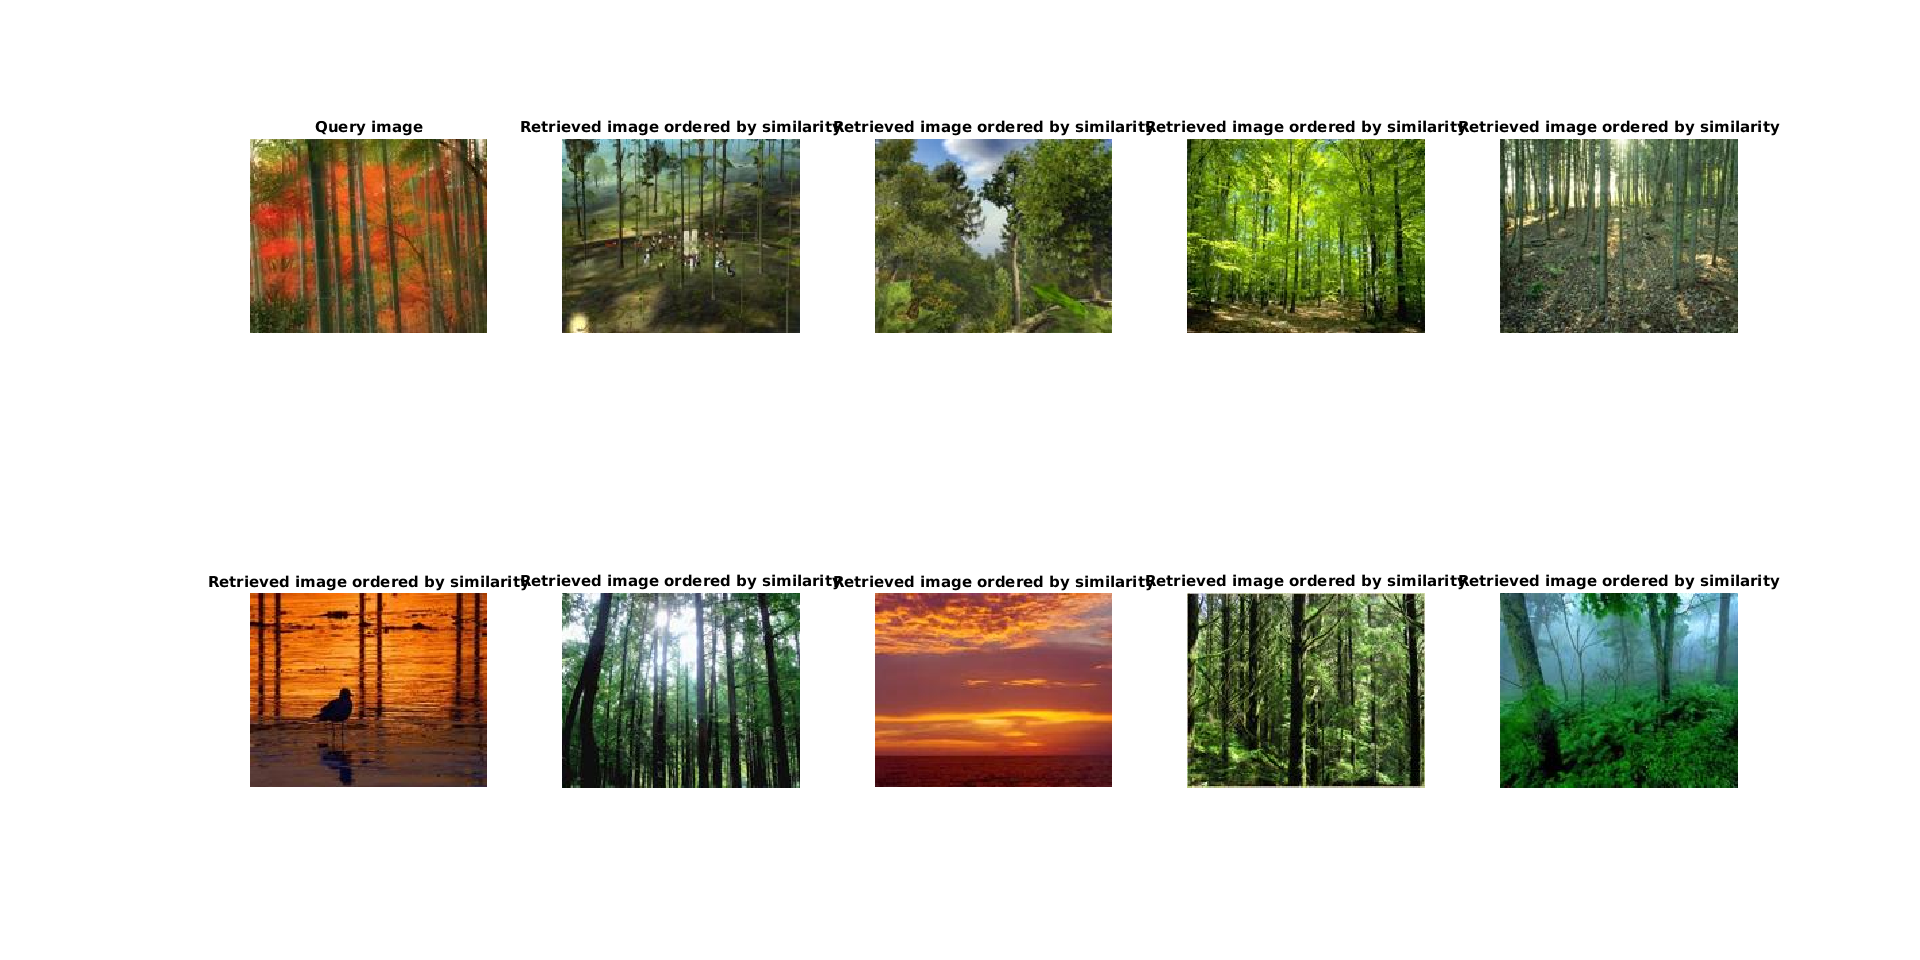
\includegraphics[width=\textwidth]{im415(2)-sinColores.png}
\end{center}

 \begin{center}
	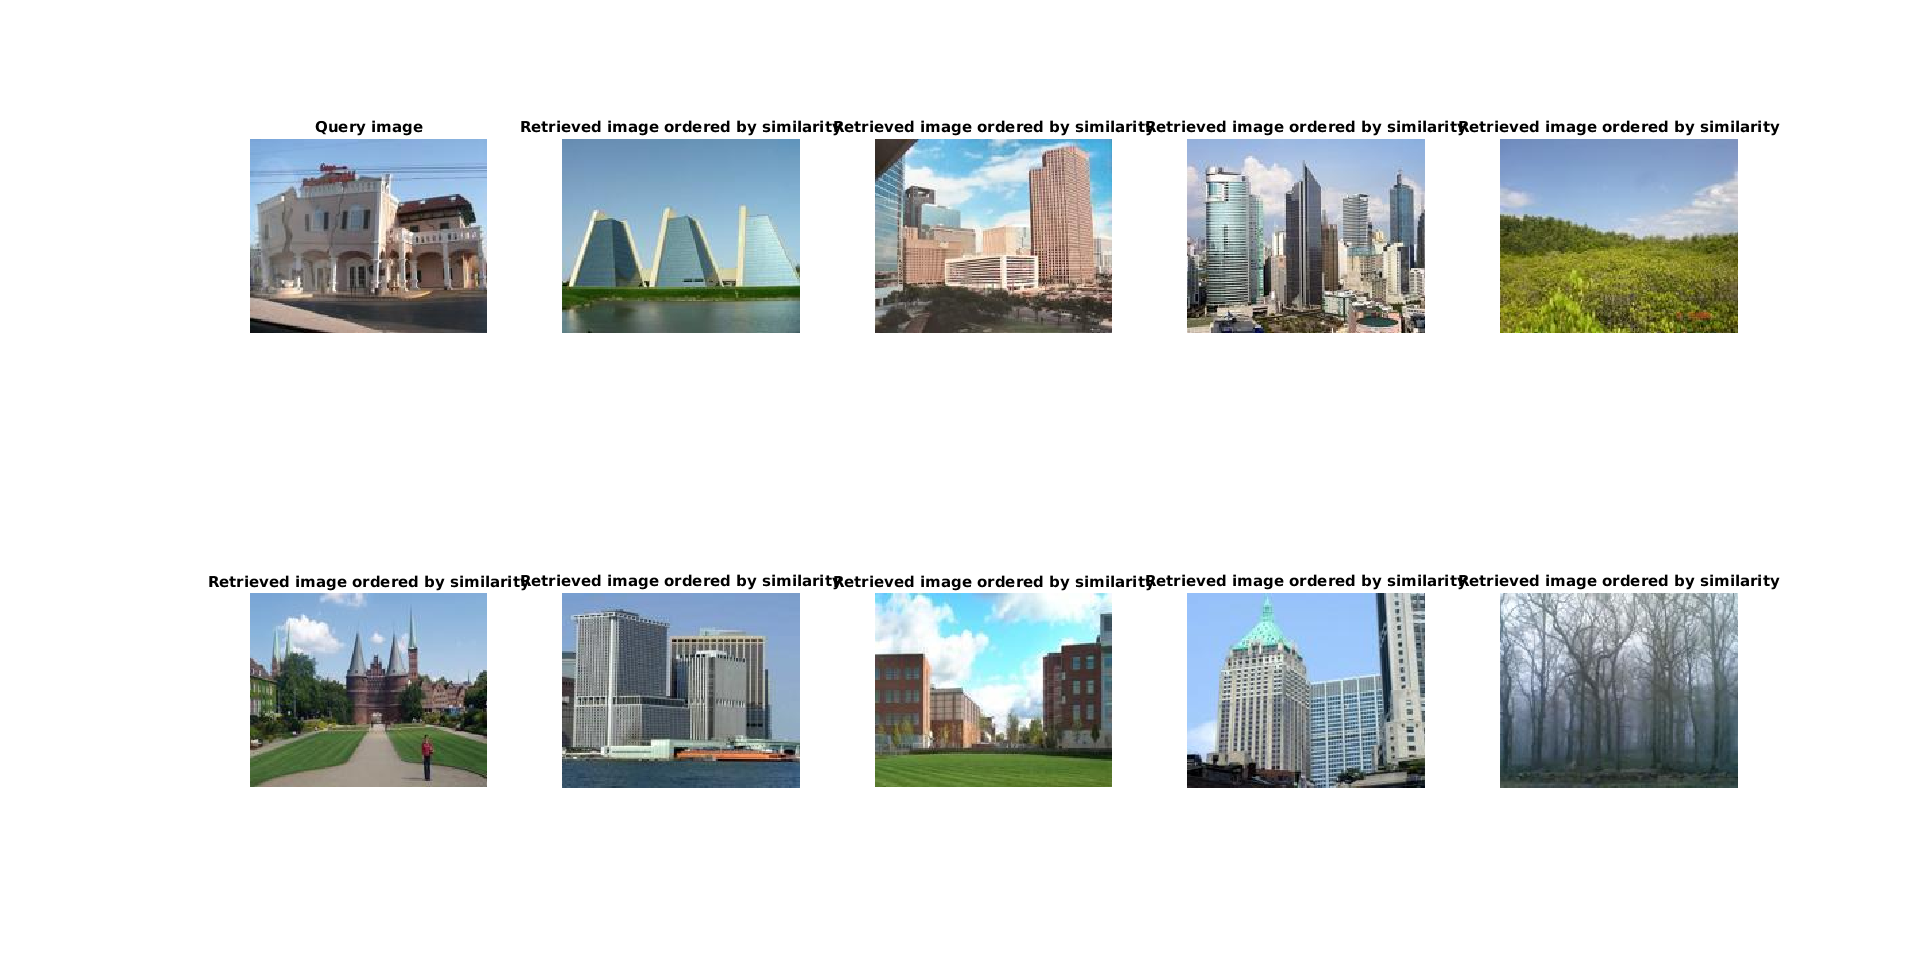
\includegraphics[width=\textwidth]{im415(3)-sinColores.png}
\end{center}

 \item \textit{Observar cómo mejora el resultado si aparte de los filtros de textura añadimos el color  (r,g,b)  como  tres  características  más  por  cada  imagen.  
 ¿Qué  dimensión tendrá el espacio de características si añadimos el color?}

 Resultado de añadiendo colores:
 
 \begin{center}
	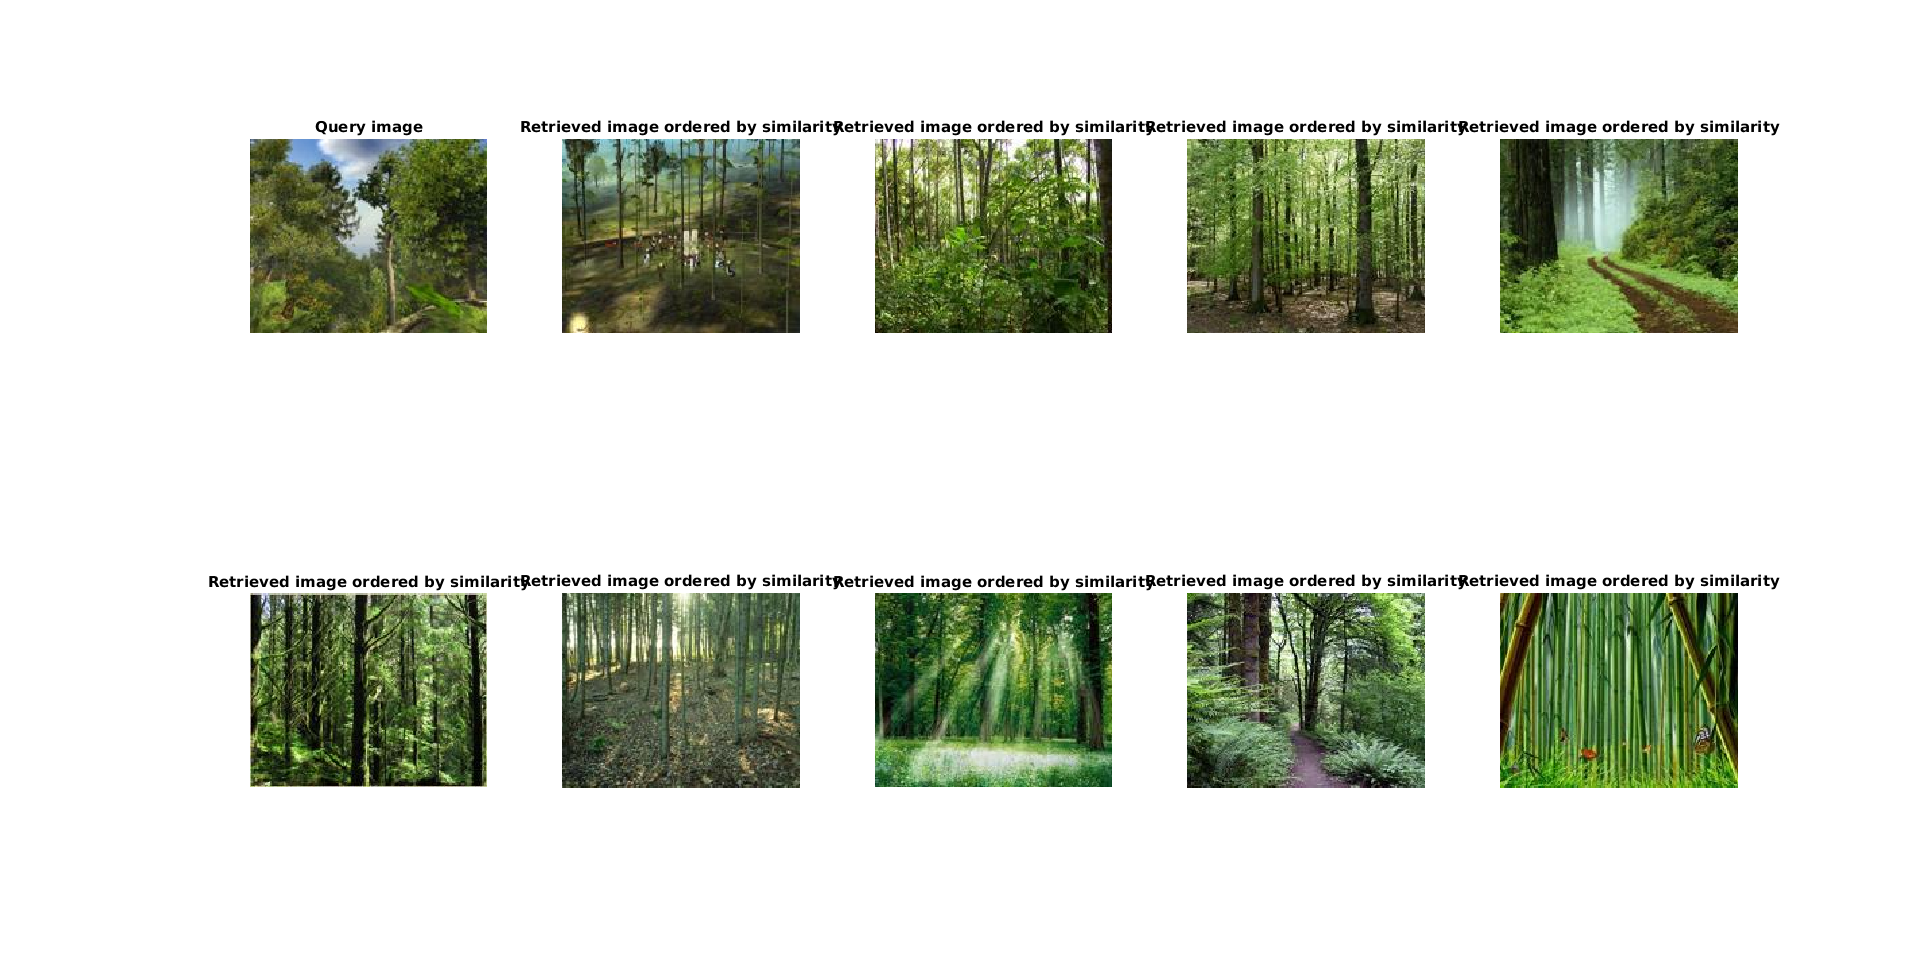
\includegraphics[width=\textwidth]{im415(1).png}
\end{center}

 \begin{center}
	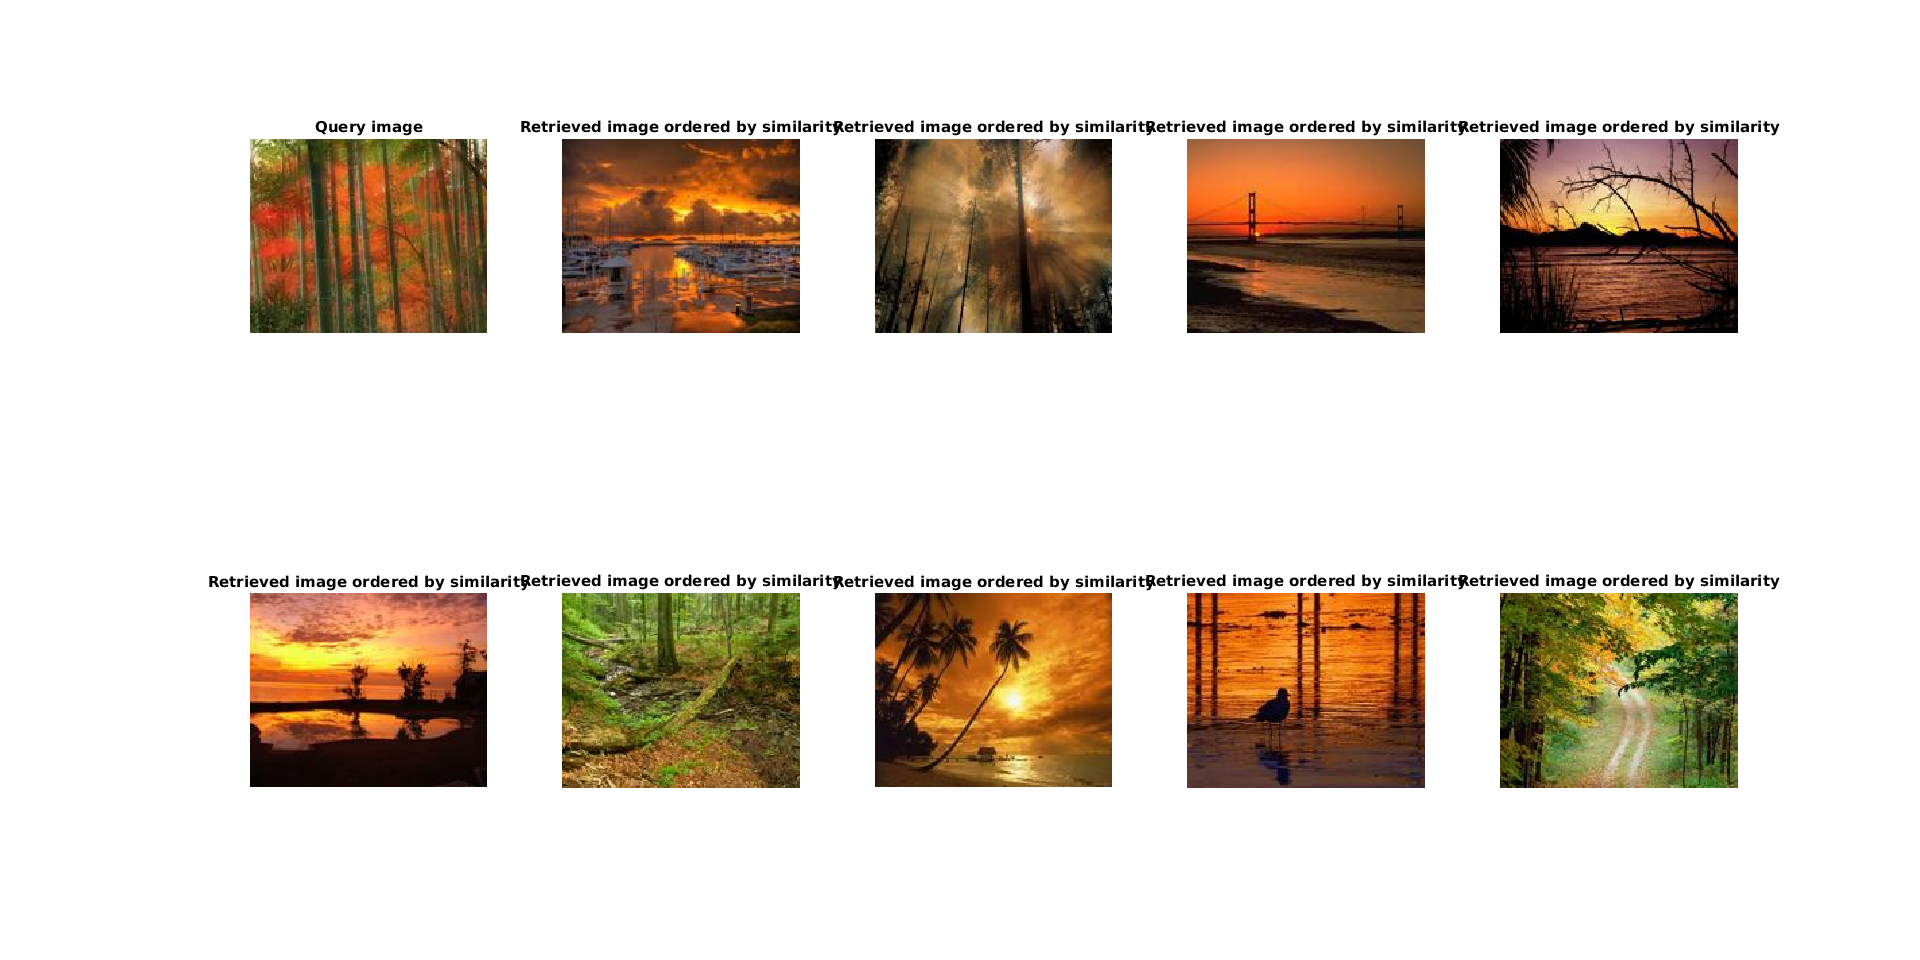
\includegraphics[width=\textwidth]{im415(2).png}
\end{center}

 \begin{center}
	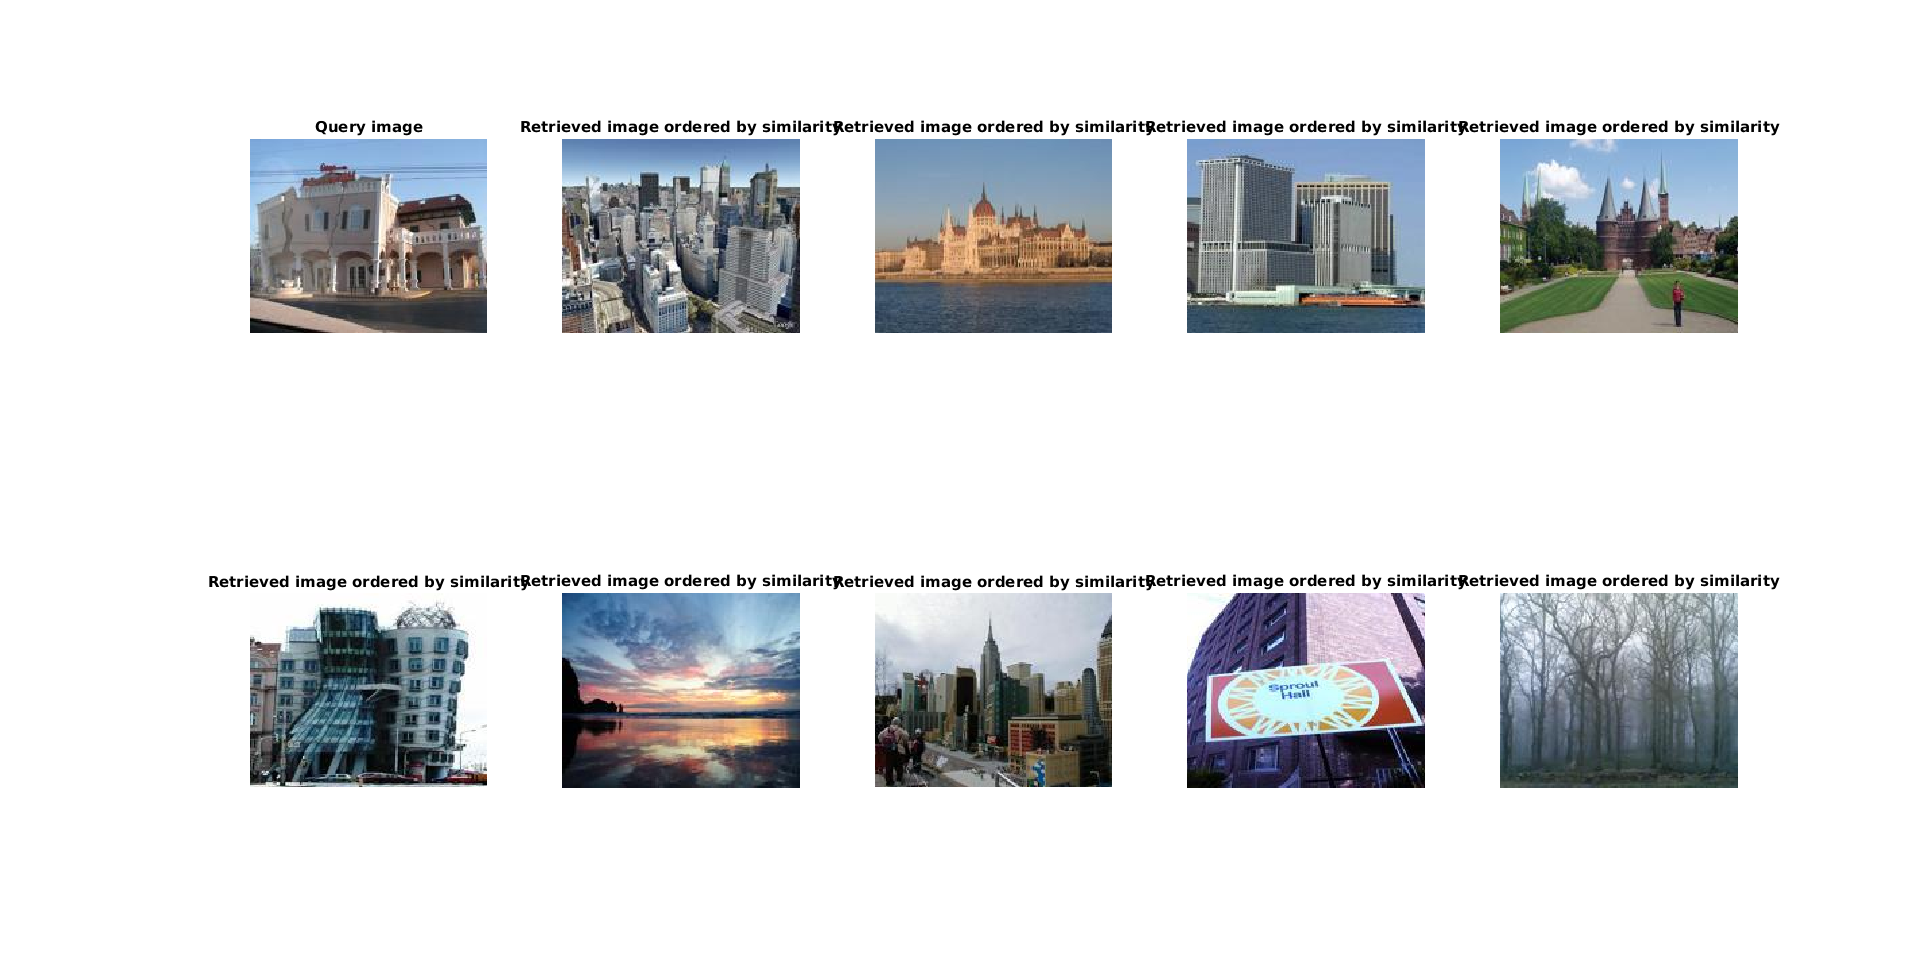
\includegraphics[width=\textwidth]{im415(3).png}
\end{center} 
 
 Tiene dimensión 48+3 = 51 si añadimos colores.
 
 \item \textit{Observa cuáles son las características más discriminativas para cada conjunto de imágenes  primero  sin  utilizar  color  y  luego  utilizando  color.  
 Comenta  tus observaciones sobre el funcionamiento del algoritmo y posibles mejoras.}

 Utilizando colores la ordenación parece más precisa que sin ella, porque sin colores solo tenemos en cuenta las formas que se encuentran en la imagen.
 Aunque con colores el color podría ser demasiado determinante en la ordenación.
 
 El rendimiento del algoritmo es sorprendentemente bueno y no se nos ocurre ninguna mejora, porque las ordenaciones parecen estar bien hechas. 
 
 \end{enumerate}

\newpage

 \item \textbf{Local binary patterns (LBP)}

 \begin{enumerate}
 \item \textit{¿Qué parámetros de entrada recibe el método vl\_lbp? ¿A qué corresponde el valor devuelto y qué dimensión tiene?}

Recibe la imagen y el número de vecinos a mirar para crear el descriptor. El valor devuelto corresponde a los histogramas de cada bloque que ha mirado, 
tiene dimensión filas de la imagen por columnas de la imagen por bloques que se hicieron (18x22x58 en caso del buildings\_1.jpg)

 \item \textit{  Implementar una  función getLBPfeatures que dada una imagen, construye un  descriptor  de  texturas  definido  como  el  histograma  promedio  
 de  los histogramas  calculados  por  la  función  vl\_lbp para cada  región analizada.  ¿Qué dimensión tiene el descriptor?}

 El descriptor tiene dimensión filas de la imagen por columnas de la imagen, pero estirado a un solo vector. En caso de buildings\_1.jpg es de 18x22 = 396.
 
 \item \textit{Utiliza la  función  retrieveKImages implementada en el ejercicio  4.1.5  utilizando como características los descriptores de textura obtenidos con LBP. 
 Compara los resultados  obtenidos en ambos  casos  (filtros Gaussianos  vs.  LBP),  y  explica las ventajas de cada uno.}

 Resultado usando LBP:
 
 \begin{center}
	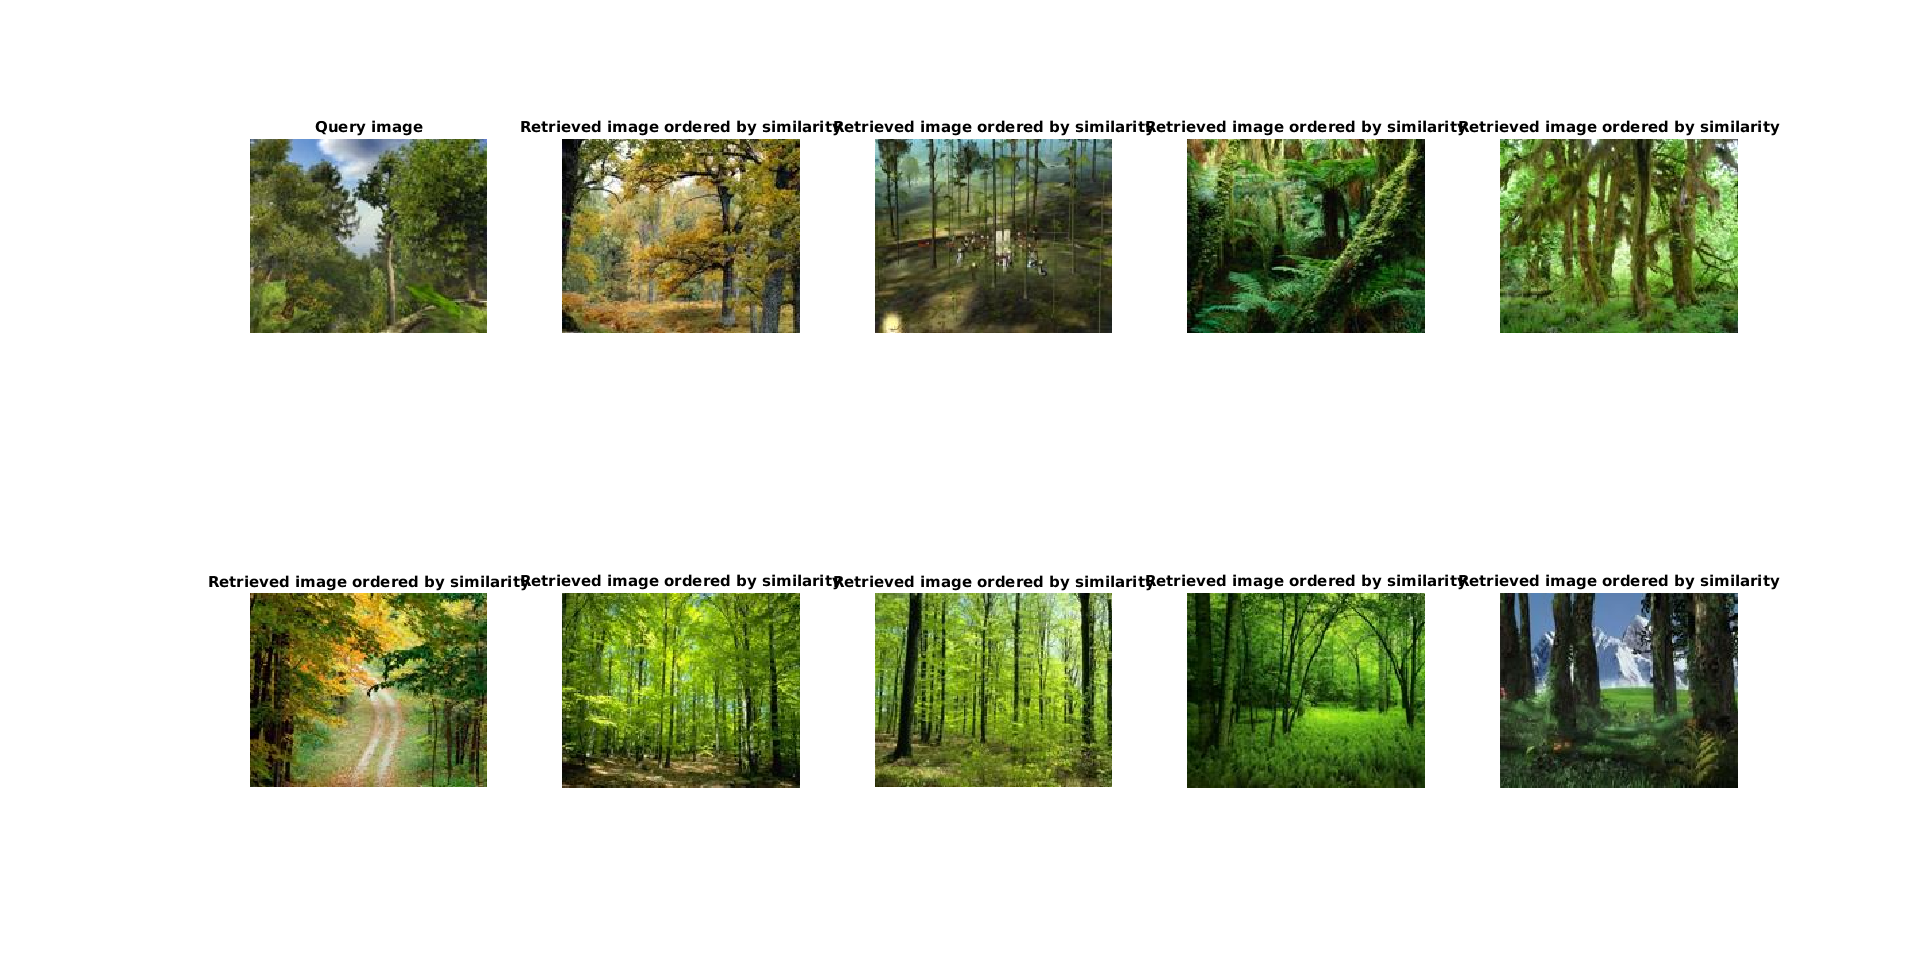
\includegraphics[width=\textwidth]{im42(1).png}
\end{center} 

 \begin{center}
	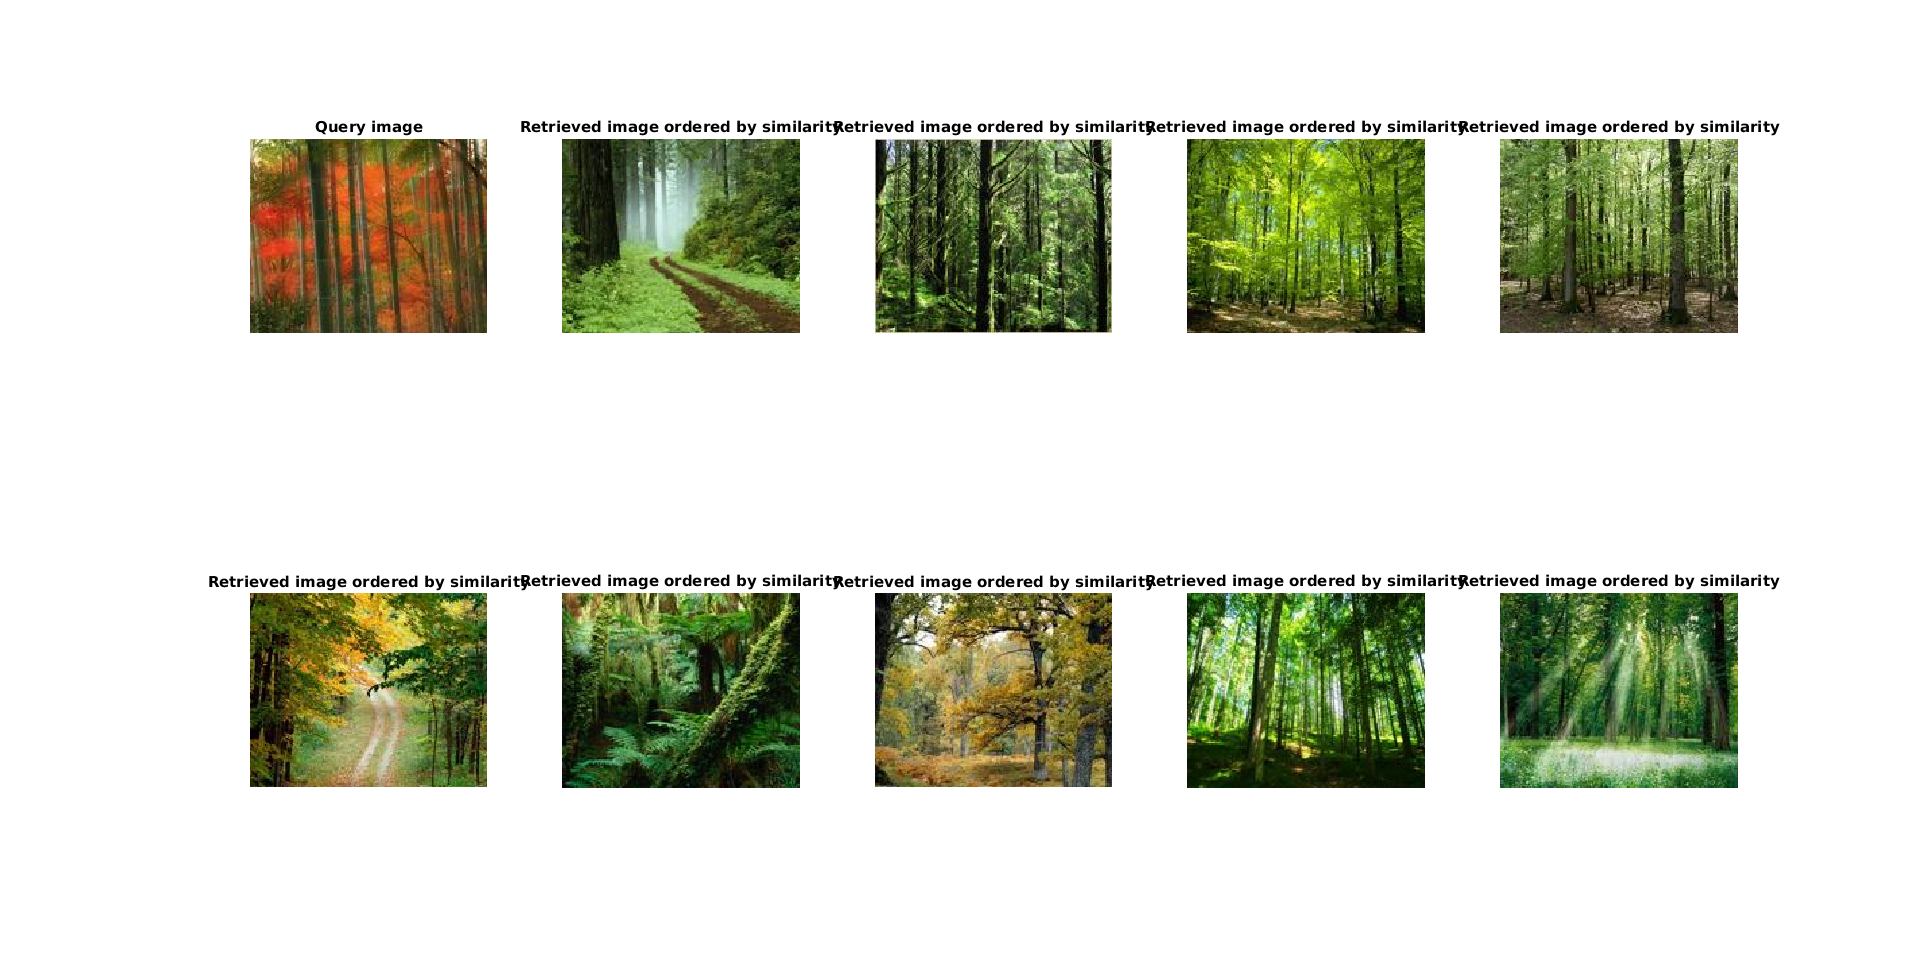
\includegraphics[width=\textwidth]{im42(2).png}
\end{center} 

 \begin{center}
	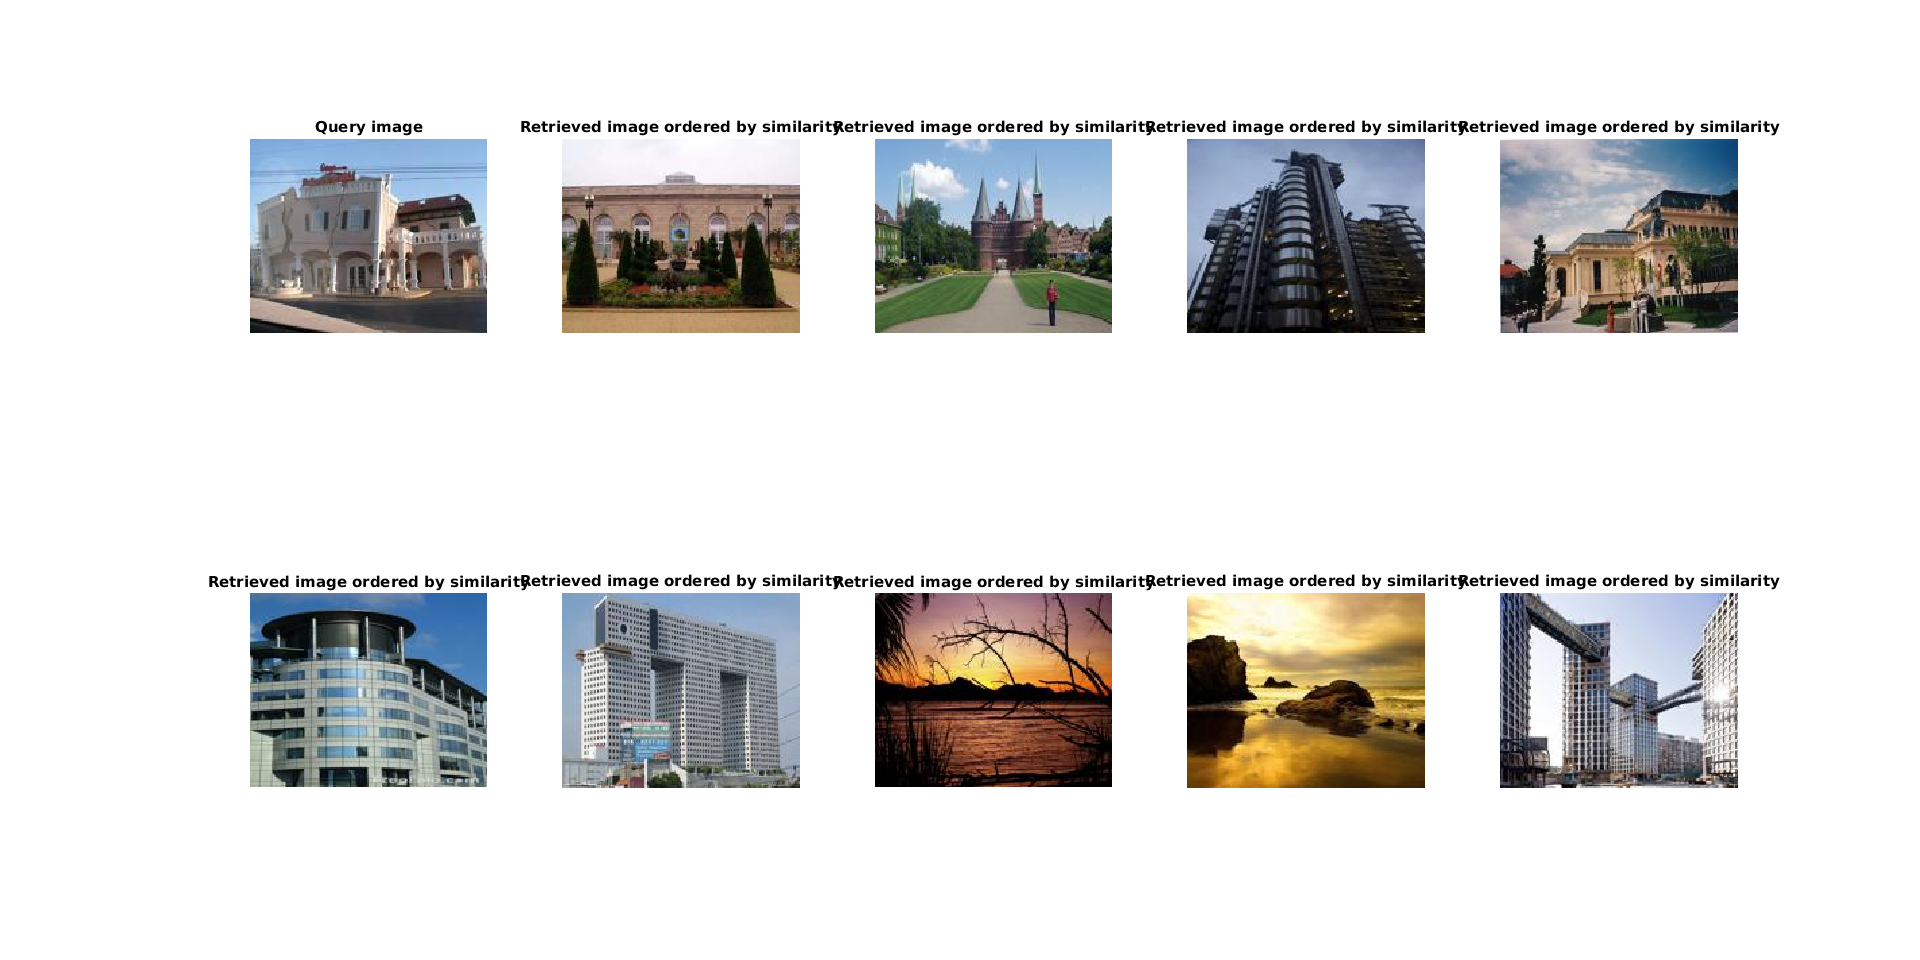
\includegraphics[width=\textwidth]{im42(3).png}
\end{center} 
 
 Con los filtros gaussianos, la ordenación de parecido funciona mejor si miramos las imágenes desde lejos y la de LBP si miramos las imágenes más ampliado.
 
 \end{enumerate}

\end{enumerate}

\end{document}